\documentclass[
    % a4paper,
    ebook,
    11pt,
    % twoside,
    oneside,
    onecolumn,
    openright,
    final
    % draft
]{memoir}

\usepackage[]{geometry}
% \usepackage[final]{microtype}
\usepackage{indentfirst}
\linespread{1.333}\selectfont

\usepackage{amsmath}
\usepackage{amsfonts}
\usepackage{amssymb}
\numberwithin{equation}{section}

\usepackage{physics}
\usepackage{tensor}

\usepackage{graphicx}

\usepackage{natbib}

\usepackage{kotex}
\usepackage{lipsum}

\usepackage{hyperref}
\hypersetup{%
    unicode=true,
    colorlinks=false
}

\usepackage{xcolor}

\usepackage[
    answers,
    % noanswers,
    final
]{probsoln}

\begin{document}

\begin{titlingpage}
	\title{\HUGE\textbf{Notes on Electrodynamics}}
	\author{\Large\textbf{Nanaki}}
	\date{\Large{\today}}

	\pagenumbering{Alph}
	\maketitle
	\begin{center}
		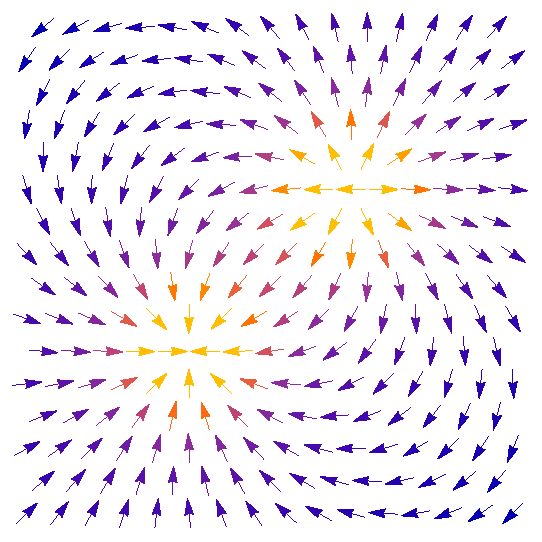
\includegraphics[width=0.65\textwidth]{figures/cover.pdf}
	\end{center}
\end{titlingpage}

\frontmatter

\tableofcontents
% \clearpage

\mainmatter

% === Introduction ===
% \part{Introduction}
% \chapter{Classical Electrodynamics and Special Relativity}


% === Special Relativiy ===
\part{The Special Theory of Relativity}

\chapter{The Principle of Relativity}

\chapter{Physical Interpretation}

\chapter{Minkowski Geometry}

\chapter{Relativistic Mechanics}

% === Classical Electrodynamics ===
\part{Fundamental Electrodynamics}

\chapter[Charges in EM Fields]{Charges in Electromagnetic Fields}
\label{ch:05a}

\section{Elementary Particles in the Theory of Relativity}
\label{sec:05a-01a}

상대론적 역학을 논하기 전에 고전역학에서 배운 내용을 생각해보자. 고전역학에서는 입자들의 상호작용(interaction)을 기술하기 위해서 장(field)을 사용한다. 좀 더 구체적으로 말하자면 입자가 주위에 장을 생성하면 다른 모든 입자가 이 장에 영향을 받아서 힘을 받게 된다. 고전역학에서 장은 입자들의 상호작용이라는 물리적인 현상을 설명하는 방식의 하나이다.
그런데 상대성 이론에서는 상호작용의 전파 속도가 유한하므로 상황이 근본적으로 다르다. 입자에 작용하는 힘은 더는 힘이 작용하는 순간 입자가 어디에 있는지만으로 결정되지 않는다. 한 입자의 위치가 변하면 그 변화는 특정 시간 간격이 지나간 후에 다른 입자에 영향을 준다. 이는 장 자체가 물리적으로 실재\footnote{동역학을 갖고 있다.}한다는 것을 의미한다. 우리는 더는 서로 멀리 떨어져 있는 입자들의 직접적인 상호작용에 대해서 말할 수 없다. 상호작용은 공간적으로 인접한 지점 사이에서 한순간에 발생할 수 있다. 따라서 우리는 한 입자와 장의 상호작용 그리고 장과 두 번째 입자의 후속 상호작용에 대해 말해야 한다.

입자와 전자기장의 상호작용을 고려하기 전에 상대론적 역학에서 입자란 무엇인지에 대해 생각해보자.
고전역학에서는 어떤 조건에서도 모양과 부피가 변하지 않는\footnote{물체 안의 임의의 두 점 사이의 거리가 일정한} 물체를 도입했다. 이를 강체(rigid body)라 부른다. 그러나 상대성 이론은 강체가 존재하지 않는다고 말한다. 증명은 간단하다. 일단 강체가 존재한다고 가정하자. 이 강체에 외력이 작용한다면 강체의 모든 지점은 힘이 가해지는 지점과 동시에 움직여야 한다. 그렇지 않으면 변형된다. 그러나 상대성 이론에 따르면 특점 지점에 가해지는 힘은 유한한 속도로 다른 지점에 전달되어 모든 지점이 동시에 움직일 수 없다. 따라서 귀류법에 따라 강체는 존재하지 않는다.

위의 논의에서 우리는 상대론적 역학\footnote{Classical (non-quantum) relativistic mechanics}에서는 기본 입자(elementary particle)는 반드시 점\footnote{물론 양자역학을 도입한다면 굉장히 어려운 문제가 된다. 불확정성 원리로부터 점 입자는 존재할 수 없다는 것을 알 수 있다.}으로 다루어야 한다는 것을 알 수 있다.

\section{Four-Potential of a Field}


\section{Equations of Motion of a Charge in a Field}
\label{sec:05a-03a}


\section{Gauge Invariance}
\label{sec:05a-04a}

고전역학에서 potential은 차이가 중요하여 임의의 상수를 더하거나 빼도 상관 없는 양이었다. Four-potential이라는 이름의 의미를 알기 위해서 운동방정식 \eqref{eq:ll1705}를 먼저 관찰해보자. 운동방정식에서 전하의 운동에 영향을 미치는 것은 potential이 아니라 장의 세기인 $\vb{E}$와 $\vb{B}$임을 알 수 있다. 따라서 4-potential이 서로 같은 장에 대응된다면 물리적으로 동등하다.

만약 potential $\phi$와 $\vb{A}$가 주어져 있다면 $\vb{E}$와 $\vb{B}$는 유일하게 결정된다. 그러나 하나의 전자기장에는 여러 potential이 대응된다. 이를 보이기 위해서 임의의 시공간 좌표에 대한 함수 $f$에 대하여 다음과 같은 변환을 생각해보자.
\begin{equation}\label{eq:ll1801}
    \tensor{A}{_\mu} \to \tensor{A}{_\mu} - \tensor{\partial}{_\mu} f
\end{equation}
이는 작용에 다음과 같은 항을 추가한다.
\begin{equation}
    q \; \dd \tensor{x}{^\mu} \; \tensor{\partial}{_\mu} f = d ( q f )
\end{equation}
그러나 이 항은 전미분이다. 따라서 운동방정식에 아무런 영향을 주지 않는다.


\section[Constant EM Field]{Constant Electromagnetic Field}
\label{sec:05a-05a}

Constant electromagnetic field는 장이 시간에 의존하지 않는다는 뜻으로 정적인 전자기장으로 번역할 수 있다. 분명히 정적인 장의 potential은 시간에 의존하지 않도록 잡을 수 있다. 이 경우에 다음이 성립한다.
\begin{equation}\label{eq:ll1901}
    \vb{E} = - \grad \phi \qquad \vb{B} = \curl \vb{A}
\end{equation}
따라서 전기장과 자기장은 각각 scalar potentail과 vector potential로 결정되며 서로 얽혀있지 않게\footnote{Decoupled} 된다.

Section \ref{sec:05a-04a}에서 potential은 유일하게 결정되지 않는다는 것을 보았다. 하지만 정적인 전자기장을 시간에 의존하지 않는 potential로 나타낸다면 scalar potential의 경우에는 오직 상수\footnote{시공간 좌표에 의존하지 않는}만을 더할 수 있다. 보통 이러한 경우 $\phi$는 공간상의 특정한 점에서 특정한 값을 갖도록 설정한다. 사실 $\lim _{r \to \infty} \phi = 0$이도록 잡는 것이 더 흔하다. 이런 방식으로 정적인 장의 scalar potential을 유일하게 결정한다.

한편 vector potential은 정적인 장에 대해서도 유일하게 결정되지 않는다. 언제나 (시간에 의존하지 않고) 공간 좌표에 의존하는 임의의 scalar 함수의 gradient를 더할 수 있다.

\section{Motion in a Constant Uniform Electric Field}
\label{sec:05a-06a}

전하량이 $q$인 전하가 균일한 전기장 $\vb{E}$ 안에서 운동하는 상황을 생각해보자. 장의 방향이 $x$축과 평행하다고 하자. 운동은 평면 위에서 이루어질 것이다. 이 평면이 $xy$ 평면이라고 하자.
그러면 운동방정식 \eqref{eq:ll1705}은 다음과 같다.
\begin{equation*}
    \dot{p_x} = q E \qquad \dot{p_y} = 0
\end{equation*}
여기서 점은 시간 $t$에 대한 미분이다.
$t = 0$일 때 $p_x = 0$이고 $p_0$가 초기 운동량이라 하자. 이 식을 적분하면 다음과 같다.
\begin{equation}\label{eq:ll2001}
    p_x = q E t \qquad p_y = p_0
\end{equation}

입자의 kinetic energy는 $T = \sqrt{m^2 c^4 + p^2 c^2}$이므로 \eqref{eq:ll2001}로 치환하고 $T_0$이 $t = 0$일때의 kinetic energy라고 한다면 다음을 얻는다.
\begin{equation}\label{eq:ll2002}
    T = \sqrt{m^2 c^4 + c^2 p_0^2 + (c q E t)^2} = \sqrt{T_0^2 + (c q E t)^2}
\end{equation}

입자의 속도는 $\vb{v} = \vb{p} c^2 / T$이므로 다음을 얻는다.
\begin{equation*}
    \dv{x}{t} = \frac{p_x c^2}{T} = \frac{c^2 q E t}{\sqrt{T_0^2 + (q e E t)^2}}
\end{equation*}
간단한 꼴을 얻기 위해서 적분 상수를 $0$이라 하고 적분하면 입자의 $x$ 좌표를 알 수 있다.
\begin{equation}\label{eq:ll2003}
    x = \frac{\sqrt{T_0^2 + (c q E t)^2}}{q E}
\end{equation}

$y$ 좌표를 알아내기 위하여 다음을 적분한다.
\begin{equation*}
    \dv{y}{t} = \frac{p_y c^2}{T} = \frac{p_0 c^2}{\sqrt{T_0^2 + (q e E t)^2}}
\end{equation*}
그 결과 다음을 얻는다.
\begin{equation}\label{eq:ll2004}
    y = \frac{p_0 c}{q E} \sinh^{-1} \left( \frac{c q E t}{T_0} \right)
\end{equation}

\eqref{eq:ll2004}를 $t$에 대하여 풀어서 \eqref{eq:ll2003}에 대입하면 다음을 얻는다.
\begin{equation}\label{eq:ll2005}
    x = \frac{T_0}{q E} \cosh \frac{q E y}{p_0 c}
\end{equation}
이로부터 균일한 전기장 안의 입자는 현수선을 따라서 운동함을 알 수 있다.

만약 입자의 속도가 충분히 작다면 $v \ll c$을 만족하고 $ p_0 = m v_0 $, $ T_0 = m c^2$라고 둘 수 있다. 이제 \eqref{eq:ll2005}을 급수 전개하고 고차항을 무시하면 다음을 얻는다.
\begin{equation*}
    x = \frac{q E}{2 m v_0^2} y^2 + C
\end{equation*}
이 식은 포물선의 방정식이다. 이 결과는 고전역학의 결과와 같다.

% Motion in a constant unifrom magnetic field
% Motion of a charge in constant uniform electric and magnetic fields
% The Electromagnetic Field Tensor
% Lorentz Transformation of the Field
% Lorentz Invariants of the Field

\chapter[The EM Field Equations]{The Electromagnetic Field Equations}
\label{ch:06a}

\section{Maxwell's Equations I}
\label{sec:06a-01}

% 

\chapter[Constant EM Fields]{Constant Electromagnetic Fields}
\label{ch:07a}

% === Electrodynamics of Continuous Media
\part{Electrodynamics of Continuous Media}

\chapter{Electrostatics of Conductors}

\chapter{Electrostatics of Dielectrics}

\chapter{Steady Current}

\chapter{Magnetostatics}

\chapter{Ferromagnetism and Antiferromagnetism}

\chapter{Quasi-Static Electromagnetic Field}

% === Electromagnetic Waves ===
\part{Electromagnetic Waves}

\chapter{Electromagnetic Waves}

\chapter{The Propagation of Electromagnetic Waves}

\chapter{The Field of Moving Charges}
% 2-VIII 8-XIV

\chapter{Radiation of Electromagnetic Waves}

\chapter{Scattering of Electromagnetic Waves}

\chapter{Diffraction of Electromagnetic Waves}
% 2-59 2-60 2-61

% === Appendices ===
\appendix
\part{Appendix}

\chapter{Mathematical Tools}
% Calculus of Variation
% Noether's Theorem
% Multipole Expansion

\backmatter

\end{document}
